%%
%% 章:TeX とその仲間
%%------------------------------------------------------------------------------------------------------------------------------%%
\chapter{\TeX{}とその仲間}
本章では\TeX{}とその仲間(\pdfTeX、\XeTeX、\LuaTeX、\pTeX、\upTeX)との関係について紹介する。
%%
%% 節:TeX とは?
%%--------------------------------------------------------------------------------------------------------------------%%
\section{\TeX{}とは?}
\TeX{}は\ruby{組版}{くみはん}ソフトである。
組版(typesetting)とは印刷用語で、活字を組んで\ruby{版}{はん}(印刷用の板)を作ることを意味する。
\TeX{}はコンピュータでテキストと図版をうまく配置して、版にあたるもの(PDF あるいは PostScript ファイル)を出力する(タイプセットする)ためのソフトウェアである。\\

\TeX{}には次のような特徴がある。
\vspc{-0.50zw}\begin{itemize}\setlength{\leftskip}{-1.00zw}%\setlength{\labelsep}{+1.00zw}
\item \TeX{}はオープンソースソフトウェアなので無料で入手することができ、自由に中身を調べたり改良することができる。商用利用も自由に行うことができる。
\item \TeX{}は Windows でも、Mac や Linux などの UNIX 系 OS でも全く同じ動作をする。すなわち、入力が同じであれば、原理的には全く同じ出力が得られる。
\item \TeX{}への入力はテキスト形式なので、普通のテキストエディタで読み書きすることができ、再利用・データベース化が容易である。
\item 自動ハイフネーション、ペアカーニング(AV や To など相補的な形の文字を食い込ませる処理)、リガチャ(fi、fl、ffi、ffl などのような\ruby{合字}{ごうじ}(対応フォントのみ))処理、独立行(ウィドウまたはオーファン)処理(段落の最初の行だけ、あるいは最後の行だけが別ページになることを抑制する処理)など、高度な組版技術が組み込まれている。
\item 特に数式の組版については定評があり、数式をテキスト形式で表す際の事実上の標準となっている。
\end{itemize}\vspc{-1.50zw}
%%
%% 節:TeX の読み方・書き方
%%--------------------------------------------------------------------------------------------------------------------%%
\section{\TeX{}の読み方・書き方}
\TeX{}の作者 \ruby{Knuth}{クヌース} 教授(Donald E. Knuth:1938 ~:計算機科学の分野で最も偉大な学者の1人)によれば、\TeX{}はギリシア語から命名したもので、最後の X は口の奥で発声する無音の「ハ」に近い音だそうだが、英語でこれに一番近い音は /k/ なので「テック」と読む人が多いようである。
ドイツ語では「テッヒ」という発音が広く用いられている。\\

日本では、特に大学関係者の間では昔から「テフ」と呼び慣わされているが、英語圏で\TeX{}を覚えた人や出版関係者の間では「テック」という発音が広く用いられている。\\

\TeX{}は見ての通り E を少し下げて字間を詰めて表記する。
このような文字の上げ下げや詰めは\TeX{}の得意とするところだが、これができない場合には TeX と表記することになっている(TEX や Tex とは表記しない)。
%%
%% 節:LaTeX とは?
%%--------------------------------------------------------------------------------------------------------------------%%
\section{\LaTeX{}とは?}
\LaTeX{}は DEC(現HP)のコンピュータ科学者 \ruby{Leslie}{レスリー} \ruby{Lamport}{ランポート}\footnote{Lamport はその後 2001 年に Microsoft Research に移籍。2013 年にはチューリング賞を受賞している。} によって機能拡張された\TeX{}である。
元々の\TeX{}と同様にオープンソースソフトとして配布されている。\\

\LaTeX{}は日本では「ラテック」あるいは「ラテフ」と読まれる。
英語圏では「\textbf{\.レ}イテック」と発音されることが多いようである(アクセントの位置を\.圏\.点付きの\textbf{太字}で示してある)。\\

最初の\LaTeX{}は 1980 年代に開発されたが、1993 年には\LaTeXe{}という新しい\LaTeX{}が開発され、今日では\LaTeX{}と言えばほぼ確実に\LaTeXe{}を指すようになっている(古い\LaTeX{}は{\LaTeX~2.09}と呼ばれる)。
本稿でも以下では\LaTeXe{}のことを単に\LaTeX{}と表記することにする。\\

\LaTeX{}は見ての通り A を小さく上付きにして表記する。
文字の上げ下げができない場合は LaTeX と表記することになっている。
同様に\LaTeXe{}と表記できない場合には LaTeX2e と表記する。\\

\LaTeX{}の特徴は、文書の論理的な構造と視覚的なレイアウトを分けて考えることができることである。\\

例えば「はじめに」という\ruby{節}{セクション}の見出しがあれば、文書ファイルに、
\vspc{+0.50zw}\begin{mdframed}[roundcorner=0.50zw,leftmargin=3.00zw,rightmargin=3.00zw,skipabove=0.40zw,skipbelow=0.40zw,innertopmargin=4.00pt,innerbottommargin=4.00pt,innerleftmargin=5.00pt,innerrightmargin=5.00pt,linecolor=gray!020,linewidth=0.50pt,backgroundcolor=gray!20]
\begin{verbatim}
\section{はじめに}
\end{verbatim}
\end{mdframed}\vspc{-0.70zw}
のように記述しておく。
この \verb'\section{...}' という命令が、紙面上のデザイン、例えば「14 ポイントのゴシック体で左寄せ、前後の空きはそれぞれ何ミリを基準とし、何ミリ以内なら伸ばしてもよい…」というレイアウトに対応するといったことは、様式・判型ごとに別ファイル(クラスファイル・スタイルファイル)に登録されている。
標準のクラスファイルのデザインが気に入らなければ、自由に変更することができる。
クラスファイルだけ変更すれば、同じ文書ファイルでも違ったレイアウトで出力することができる。\\

仮に、文書ファイルに「ここは 14 ポイントのゴシック体で 3 行どり中央に…」などと書き込んでしまっては、後で組み方を変更しようとする際に原稿全体に手を入れなければならない。
下手をすると、節ごとに見出しの体裁が違ってしまうことにもなりかねない。
文書の再利用も難しくなる。\\

更に、\LaTeX{}は章・節・図・表・数式などの番号を自動的に付けてくれるし、参考箇所には番号やページを自動挿入することができる。
目次・索引・引用文献の処理まで自動的に行われる。
また、\ruby{柱}{はしら}も自動的に作成される。\\

このような便利な機能を備えるため、\LaTeX{}利用者が飛躍的に増え、\TeX{}を使っているといっても実際には\LaTeX{}であることが多くなっている。\\

\LaTeX{}は\TeX{}のプログラミング機能(マクロ機能)を用いて作られたものである。
一方、\TeX{}本体(マクロと区別するためにエンジンと呼ぶことがある)も改良され、特に日本では日本語の扱いに優れた\pTeX{}というエンジンが広く用いられている。
\pTeX{}用にマクロを修正した\LaTeX{}が\pLaTeX(\pLaTeXe)である。\\

\LaTeX{}は理系の論文や本の製作に広く用いられている。
多くの論文誌や \ruby{arXiv}{アーカイブ}(http://arxiv.org)のようなプレプリントサーバは\LaTeX{}での論文投稿を推奨しており、理系の出版社は多くの本を\LaTeX{}で製作している。
一例を挙げれば『岩波数学辞典』の最新版(第 4 版)は全て\LaTeX(\pLaTeXe)で製作されている。\\

Wikipedia も数式は\LaTeX{}形式で記述することができる(実際には Wikipedia サーバ上の\LaTeX{}で数式部分を組版して画像に変換している)。
%%
%% 節:TeX の処理方式
%%--------------------------------------------------------------------------------------------------------------------%%
\section{\TeX{}の処理方式}
一般のワープロソフトと異なり、\TeX{}は高度な最適化を行うため、段落の最後に 1 文字追加するだけで段落の最初の改行位置が変わることもあり得る。
このような処理を、キーボードから 1 文字入力するごとに行うのはかなりのマシンパワーを必要とする。
そのため、\TeX{}ではキーを打つたびに画面上の印刷結果のイメージを更新する方式\footnote{画面表示と印刷イメージが同じ(What You See is What You Get)という意味で \ruby{WYSIWYG}{ウィジウィグ} 方式と呼ぶことがある。}ではなく、一括して全体を処理するバッチ処理方式を採用している。\\

伝統的な作業手順では、原稿は自分の使い慣れたソフト(テキストエディタ等)で記述し、テキストファイルとして保存しておく。
これを後で\LaTeX{}で一括処理する。\\

例えば、\LaTeXe{}では、
\vspc{+0.50zw}\begin{mdframed}[roundcorner=0.50zw,leftmargin=3.00zw,rightmargin=3.00zw,skipabove=0.40zw,skipbelow=0.40zw,innertopmargin=4.00pt,innerbottommargin=4.00pt,innerleftmargin=5.00pt,innerrightmargin=5.00pt,linecolor=gray!020,linewidth=0.50pt,backgroundcolor=gray!20]
\begin{verbatim}
\documentclass{jsarticle}
\begin{document}
これはサンプルの文書である。
テキストファイル中では、
どこで改行しても構わない。
印刷結果の改行位置は自動的に決定される。

段落の切れ目には空の行を入れておく。
\end{document}
\end{verbatim}
\end{mdframed}\vspc{-0.70zw}
のようなテキストファイルを入力すると、
\vspc{+0.50zw}\begin{mdframed}[roundcorner=0.50zw,leftmargin=3.00zw,rightmargin=3.00zw,skipabove=0.40zw,skipbelow=0.40zw,innertopmargin=4.00pt,innerbottommargin=4.00pt,innerleftmargin=5.00pt,innerrightmargin=5.00pt,linecolor=gray!100,linewidth=0.50pt,backgroundcolor=gray!00]
   これはサンプルの文書である。
  テキストファイル中では、
  どこで改行しても構わない。
  印刷結果の改行位置は自動的に決定される。

   段落の切れ目には空の行を入れておく。
\end{mdframed}\vspc{-0.70zw}
のように出力される(\verb'\' で始まる行は\LaTeX{}の命令である)。\\

テキストファイルを用いることの利点は多数存在する。
\vspc{-0.50zw}\begin{itemize}\setlength{\leftskip}{-1.00zw}%\setlength{\labelsep}{+1.00zw}
\item 文書入力は自分の使い慣れているソフトで行う方が楽である。どんな文書入力ソフトでもテキストファイルで保存することができるので、\TeX{}は入力ソフトを選ばない。
\item テキストファイルはコンピュータの機種に依存しない。どんなコンピュータや携帯端末でも、テキストファイルなら安全にやり取りすることができる。
\item テキストファイルの変換は容易である。そのため、データベース出力や Web フォーム入力、XML 文書などから\TeX{}に変換して組版するといったことがよく行われている。
\item テキストファイルで文書を用意する方が、コンピュータのパワーユーザの心理に適っているかもしれない。数式を考えなければ Adobe InDesign のようなリアルタイムで\TeX{}同様の処理を行うレイアウトソフトが存在するし、数式を考えても WYSIWYG な数式エディタが存在する。しかし、これらは今のところ\TeX{}に置き換わりそうにない。
\end{itemize}\vspc{-1.50zw}
%%
%% 節:TeX の出力
%%--------------------------------------------------------------------------------------------------------------------%%
\section{\TeX{}の出力}
元々の\TeX{}は、組版結果を \ruby{dvi}{ディーヴィーアイ} ファイルという中間ファイルに書き出す。
dvi は \underline{d}ev\underline{i}ce \underline{i}ndependent(装置に依存しない)という英語の略である。
この dvi ファイルを読み込んでパソコンの画面、各種プリンタ・写植機、及び PostScript や PDF などのファイルとして出力するための専用ソフト(dvi ドライバ・dvi ウェア)が、出力装置や出力ファイル形式ごとに用意されている。
特に、画面出力用の dvi ドライバのことを dvi ビューアという。\\

この処理の流れを図示すると、次のようになる。

\vspc{-5.00pt}\begin{figure}[H]\centering\scalebox{1.00}{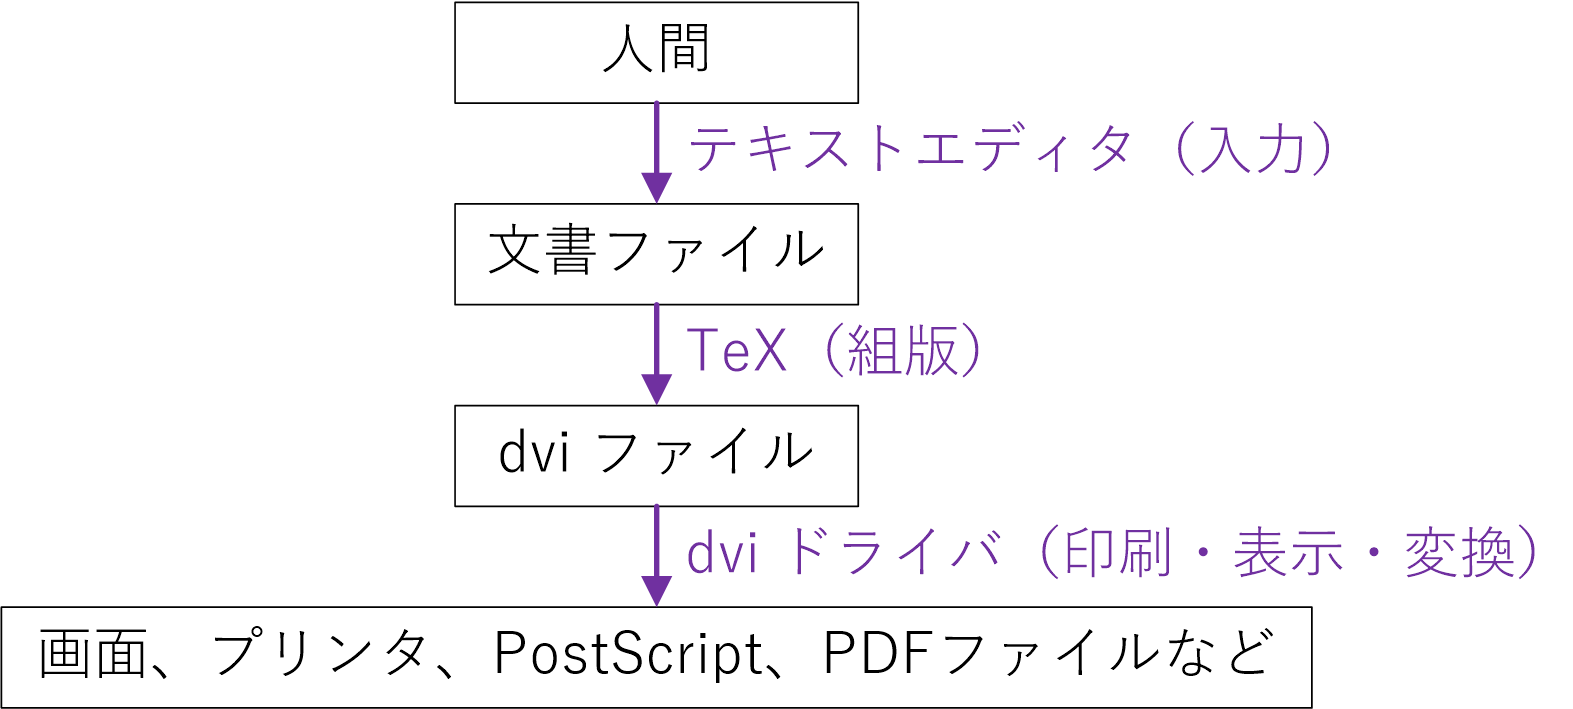
\includegraphics{./Fig/Fig01_01.PNG}}\end{figure}\vspc{-5.00pt}

ところが欧米語圏では、後述する\pdfTeX{}や\XeTeX{}、\LuaTeX{}の登場によって、\TeX{}から直接 PDF ファイルを出力することができるようになり、画面表示や印刷も全て PDF を通じて行うのが普通となっている。\\

日本語圏で広く用いられている\pTeX{}や\upTeX{}については PDF を直接出力することはできないが、dvipdfmx という高速な dvi ドライバと組み合わせて PDF を作成することができる。
%%
%% 節:TeX と日本語
%%--------------------------------------------------------------------------------------------------------------------%%
\section{\TeX{}と日本語}
日本語の文字数は非常に多く、多数のフォントに分割すれば\TeX{}でも扱えないこともないが、非常に厄介である。\\

本格的に\TeX{}を日本語化する試みはいくつか存在したが、今日広く使われているのは、かつての株式会社アスキーが開発した\ruby{\pTeX}{ピーテック}、及びそれを Unicode 対応にした\upTeX(田中琢爾{\small 氏}作)である。\\

日本語であれば文字は全て同じ幅なので単純に組んでいけばよいかというと、そうはいかない。
次のような処理が必要となる。
\vspc{-1.00zw}\begin{itemize}\setlength{\leftskip}{-1.00zw}%\setlength{\labelsep}{+1.00zw}
\item 句読点、終わり括弧(閉じ括弧)類、中黒(・)、繰返し(々ゝ)、感嘆符(!)、疑問符(?)が行頭に来ないようにする必要がある(行頭禁則処理)。促音文字(っ)、拗音文字(ゃゅょ)、長音記号(ー、音引き)などもなるべく行頭に来てほしくない。
\item 同様に、始め括弧(開き括弧)類が行末に来ないようにする必要がある(行末禁則処理)。
\item 括弧類、句読点が行頭、行末に来たときや、括弧類、句読点が連なったとき、空白が空きすぎて見えるので、詰める必要がある。
\item 段落の最後の 1 文字と句読点になるのは、なるべく避けたいところである(文字ウィドウ処理)。
\end{itemize}\vspc{-0.80zw}
これらの条件を満足するためには、文字の間隔を微調整しなければならない(詰め処理、伸ばし処理)。
しかし、調整しすぎると文字の間隔が揃わず、かえって見苦しくなってしまう。
例えば、拗促音文字(ゃゅょっ)はなるべく行頭に来ないほうがよいし、文字ウィドウもなるべく避けたいところだが、あまり厳密にこれらのルールを当てはめるとかえって不自然になることがある。
そこで \pTeX{}では、どの文字が行頭に来ると何点減点、行末に来ると何点減点、文字ウィドウは何点減点、文字の間隔がどれだけ伸びると何点減点といった具合に点数を計算し、減点の合計が最小になるように組む。
点数の配分は自由に調整することができる。\\

\pTeX{}の日本語組版が非常に優れているため広く使われるようになった一方、海外で普及している\XeTeX{}や\LuaTeX{}を日本語で扱うための仕組みも次第に改良されてきている。
%%
%% 節:TeX のライセンス
%%--------------------------------------------------------------------------------------------------------------------%%
\section{\TeX{}のライセンス}
\TeX{}関連のソフトウェアは全てオープンソースのライセンスで配布されており、商用利用も含めて自由に使うことができる(詳しくは各ソフトウェアのオンラインドキュメントを参照)。
ターミナルに「\texttt{texdoc \textcolor{blue}{ソフトウェア名}}」と打ち込めばオンラインドキュメントが表示される。\\

オリジナルの\TeX{}は、付加価値を付けたものを有償で販売することも自由である。
但し、\TeX{}と完全な互換性を持たないものは\TeX{}と名乗ることを禁止されている。
米国での\TeX{}の商標は American Mathematical Society(米国数学会)が登録しているが、これは無関係な人物に商標登録されることを防ぐためであり、\TeX{}を使う際に「\TeX{}は…の商標です」などと断る必要はない。\\

\LaTeX{}は LPPL(\LaTeX{} Project Public License, https://www.latex-project.org/lppl/)に従い、ファイル名さえ変えなければ改変したものの再配布も自由である。\\

\pLaTeX{}等については、かつての株式会社アスキーが開発したものだが、日本語\TeX{}開発コミュニティ(https://texjp.org)による「コミュニティ版」に移行している。
これらは(修正)BSD ライセンスに従っており、オリジナルの著作権表示などを残す限り改変・再配布は自由である。
%%
%% 節:TeX のディストリビューション
%%--------------------------------------------------------------------------------------------------------------------%%
\section{\TeX{}のディストリビューション}
\TeX{}は Pascal をベースとした Knuth 教授の WEB\footnote{World Wide Web の Web とは無関係である。} という「文芸的プログラミング」ツールで作成されているが、UNIX 上では通常は C 言語に変換してからコンパイルされる。\enlargethispage{+0.40zw}
これが現在の多くの\TeX{}の実装の起源である Web2c の由来である。\\

この Web2c をベースに Thomas Esser が集大成した te\TeX{}という\TeX{}ディストリビューション\footnote{ディストリビューションとは、配布用にパッケージされたソフトウェア群のことである。}が広く使われるようになり、日本では村上展之{\small 氏}がこれに基づく ptetex を配布していた。\\

一方、Windows では角藤亮{\small 氏}の W32\TeX{}というディストリビューションが広く使われるようになった。\\

その後、\TeX{}~Live という超巨大な集大成が広く使われるようになり、土村{\small 氏}もこれに基づく ptexlive を開発した。
これが現在では全て \TeX{} Live 本体に取り込まれている。
%%
%% 節:これからの TeX
%%--------------------------------------------------------------------------------------------------------------------%%
\section{これからの\TeX{}}
最初の\TeX{}が開発されたのは 1978 年である。
これだけ長い間安定して使われているソフトウェアは他に例を見ない。
\TeX{}は組版の歴史における 1 つの\ruby{不動点}{フィックスポイント}と言えるだろう。\\

しかし、既存の\TeX{}に満足していては進歩がない。
今日に至るまで、\TeX{}本体(エンジン)及びマクロに、いろいろな拡張が行われている。
エンジンの拡張としては次のようなものが挙げられる。
\vspc{-0.50zw}\begin{itemize}\setlength{\leftskip}{-1.00zw}%\setlength{\labelsep}{+1.00zw}
\item \ruby{$\epsilon$}{イー}-\TeX(e-TeX)は、\TeX{}の種々のレジスタ(変数)の個数を拡張(256 個→ 32768 個)した他、右から左に組む機能などを追加したものである。現在では \pTeX{}をはじめ殆どのシステムが $\epsilon$-\TeX{}拡張を含んでいる。\LaTeX{}パッケージにも $\epsilon$-\TeX{}拡張を仮定したものが増えている。
\item \TeX{}を日本語化した\pTeX{}も、北川弘典{\small 氏}により$\epsilon$-\TeX{}拡張された($\epsilon-$\pTeX:e-pTeX)。
\item 田中琢爾{\small 氏}の\upTeX(upTeX:読み方はユーピー\TeX{}またはユプ\TeX)は、($\epsilon-$)\pTeX{}の内部を Unicode 化したものである。
\item H\`{a}n Th\'{\^{e}} Th\`{a}nh 作の\pdfTeX(pdfTeX)は、\TeX{}の出力形式を dvi ではなく PDF にし、$\epsilon$-\TeX{}と同様の拡張を加えて、microtypography という高度な組版アルゴリズムを組み込んだものである。現在では、オリジナルの\TeX{}を置き換えて広く用いられている。
\item Jonathan Kew 作の \ruby{\XeTeX}{ズィーテック}(XeTeX)は元々 Mac の OS X 上で動作し、OS X 上の OpenType フォントをそのまま利用することができ、PDF を出力する\TeX{}だが、 Windows や Linux にも移植されている。
\item \ruby{Lua}{ルア}\TeX{}は\pdfTeX{}に軽量スクリプト言語 Lua を組み込んだものである。Unicode 対応で、\XeTeX{}とは別な(OS に依存しない)方法で OpneType フォントに対応している。\pdfTeX{}の後継として今最も注目されているものである。\LuaTeX{}-jp プロジェクトの成果と組み合わせれば\pTeX{}に置き換えて使うことができる(但し、実行速度がやや遅いのが難点である)。2005 年から開発が始まり、2016 年 9 月末にバージョン 1.0 がリリースされた。ただ、開発者たちは\LaTeX{}ではなく後述の Con\TeX{}t を主に使っているため、\LuaTeX{}の仕様が変わって\LaTeX{}で問題が生じるといったことが過去に多々あった。
\item Clerk Ma による\pTeX{}-ng は、Web2c ベースではなく C 言語で開発された Y\&Y~\TeX{}から出発して\pTeX、\upTeX{}の機能を取り込んだもので PDF を直接出力するが、まだまだ開発中のものである。
\end{itemize}\vspc{-0.50zw}
一方、\TeX{}のマクロも\LaTeXe{}ができてもう 20 年経過している。
現在では\LaTeXe{}後継の\LaTeX{}3 の開発が(気長に)行われているところである。
また、\LaTeX{}と全く異なるマクロパッケージ \ruby{Con\TeX{}t}{コンテクスト}(作者は Hans Hagen)も特にヨーロッパでユーザ層を広げている。
最新の Con\TeX{}t は\LuaTeX{}上で動作する。\\

Web 上で\LaTeX{}とほぼ互換の数式組版機能を Javascript、CSS、Web フォントで実現したものとして MathJax というものが存在する。
Web ベースの帳票印刷システムでも、サーバ側で\TeX{}経由で PDF を作成し、クライアント側で印刷するといった用途で\TeX{}が用いられることがある。\\

最近では、Markdown という非常に簡単な形式で文書を記述し、必要に応じて\LaTeX、HTML などに変換しようという流れがある。多様な形式間を相互変換する pandoc などのツールも開発されている。\\

高度な組版から PDF 作成まででき、Adobe-Japan1-{6} の 2 万字(更には IPAmj フォントの 6 万字)を使いこなせるフリーソフトウェアは、今のところ\TeX{}しか存在しない。\enlargethispage{+0.40zw}
他のソフトウェアの組版エンジンとしても、色々使いこなせると思われる。
